% Native-results integration, 2026-09-21, from verified saved reports.
% External population; never pool with v2 evidence.
% Frozen v5 native plans and source-v4 bounded-completion policy.
\section{External Extension: Evidence Before Execution}
\label{sec:tau-extension}

Repeatable behavior and sufficient grounds for authorization are distinct:
a stable route can omit the same prerequisite. We extend DFAH's eligibility
and comparability principle from recorded decisions and paths to the chain
from evidence through permission to execution and effect. The banking
intervention asks whether a semantic check reduces unsupported approvals while
preserving permitted actions and native task completion. Its interactive
population and protocol remain separate from the v2 replay evidence.

The practical question is whether a check helps the agent act on adequate
grounds and finish legitimate work at an acceptable cost. We therefore track
what evidence the gate saw, what it permitted, what actually ran and whether
the task succeeded. These measurements can move in opposite directions:
a gate can repeat its answer reliably while overlooking a missing fact or
blocking an action that the policy permits.

\paragraph{One qualification principle, two experimental regimes.}
Identical-input replay pairs decision and path agreement on a shared
denominator; interactive intervention qualifies boundary observations and
native outcomes within matched task bundles. Decisions record verdicts;
paths distinguish proposals, dispatch and completed invocations; gate evidence
contains delivered policy, dialogue and tool results. A captured record may
lack a prerequisite. Unavailable traces remain missing, observed-empty paths
require capture, and infrastructure failures leave native outcomes unknown.
The historical evidence-contact metric remains omitted.

\paragraph{Native environment and matched interventions.}
We use Sierra's $\tau$-Knowledge \texttt{banking\_knowledge}
environment~\citep{shi2026tauknowledge}, distributed in the $\tau^3$-bench
codebase under the \texttt{tau2-bench} repository name. Commit
\texttt{b7ea9074c1cb} pins the adaptive user simulator, tools, policies and
native evaluators; its inventory contains 97 tasks and 698 knowledge
documents.\footnote{Pinned source:
\url{https://github.com/sierra-research/tau2-bench/tree/b7ea9074c1cba482b30687fecdb5c8425fd6f619}.}
Primary \texttt{golden\_retrieval} supplies task-relevant documents; BM25 is
a separate exploratory condition. All arms share generator, simulator,
graders and structural checks of callable arguments, mutation metadata and
policy presence. A uses structural checks alone; B adds the generator
model's \emph{allow/block/review} judgment; C substitutes a typed-choice
API. B generates a schema-constrained JSON decision; C returns a choice and
class probabilities.\footnote{Jev is the implemented typed-choice service;
\url{https://docs.typesafe.ai/api}; \url{https://docs.typesafe.ai/models}.}
The estimand compares the implemented admission, model/API and recovery bundles.

Both gates receive the same raw projection of policy, visible dialogue, tool
results, resolved proposal and textual generator rationale, excluding hidden
criteria, reference actions and observer snapshots. The rubric assigns block
to established disqualifiers, otherwise review to missing required evidence,
and allow to supported prerequisites. Customer-supplied proof requires its
own provenance even when database facts agree. Method review was
model-assisted; human action-gold adjudication remains outstanding.

\paragraph{Execution and accounting contract.}
OpenRouter routes generator, simulator, native LLM-grader and B-gate calls
through \path{/api/v1/chat/completions}; Jev uses
\path{/api/v1/systemone}.\footnote{OpenRouter
\href{https://openrouter.ai/docs/guides/routing/provider-selection}{provider-routing documentation}
and \href{https://openrouter.ai/docs/guides/community/typesafe-sdk}{TypeSafe integration}.}
The primary bundle specifies DeepSeek v4.1 Flash/DeepInfra for generation
and B gating, Gemini 3.8 Flash/Google AI Studio for simulation and grading,
and \texttt{typesafe/jev-1.13-20260917}/TypeSafe. Chat requests restrict
providers, disable fallbacks, require parameter support and cap prices;
SystemOne receives model, state and questions. Returned identities are
checked. Requests are nonstreaming, without automatic retries or redirects,
and retain the 120-second socket timeout. A durable ledger reserves against
the supplied \$80 all-in campaign ceiling, distinguishing credit debits,
BYOK upstream costs and reconciliation bases. Retained records bind request
and response hashes, identifiers, latency and available cache metadata.

Dispatch wrapping resolves discoverable wrappers and checks eligible assistant
mutations. User actions remain native; reads and spoken disclosures are outside
this boundary. Block and review withhold execution with identical generic
feedback and at most two recoveries; completed human review is outside the
workflow. Events distinguish proposals, verdicts, dispatches, results and
effects. Database changes and in-memory capability grants have separate
hashes; wrapper audit writes are distinct from business mutations, and
occurrence identifiers distinguish repeated identical requests.

Native DB and action evaluators receive an \emph{execution view} excluding
denied calls and synthetic replies. Scoring criteria are unchanged;
communication and language graders receive original dialogue. Tool completion,
native success and per-action policy compliance remain distinct endpoints.
Frozen native plans use the upstream
\texttt{enforce\_communication\_protocol=false}: mixed messages route to the
environment while their text remains available to communication scoring.
Earlier strict-cohort failures remain configuration diagnostics.

Under source-v4 bounded completion, a generator or simulator response ending
with \texttt{finish\_reason=length} and no usable text or tool call terminates
that participant as a native agent/user error. Its valid prefix receives native
failure reward zero; raw completion and cost remain recorded. Partial usable
completions retain their classification; other malformed responses and
transport failures remain infrastructure errors. Both gates share a
90,000-byte state-plus-question admission envelope: oversize input produces
operational review without a model decision or call. This heuristic differs
from Jev's 32k-token per-question limit. Admission exclusions, parse failures
and categorical answers remain separate; unverified caching limits repeats
to observational agreement.

\paragraph{Completed native cohorts.}
The pre-collection plan requires complete B/C task bundles for the primary
two-sided sign-flip test at $\alpha=0.025$; only rejection opens the secondary
Holm(2) family.\footnote{Retained \path{V3_STATISTICAL_PLAN.md}, final prospective
declaration and missing-outcome rule, frozen through amendments 06--07.}
All 1,080 scheduled episodes produced terminal artifacts; 1,033 have evaluable
native outcomes and 47 retain unknown outcomes. The frozen cohorts use Gemini
as simulator and grader, with output limits of 8,192 tokens for generation
and 4,096 for B's gate, simulator and grader. Each task received a random arm
permutation over fixed trial bundles; a separate seed shuffled execution order.
The table reports successes/known/unknown outcomes in each arm. Tasks and
trials determine the scheduled denominator per arm. The first row is primary;
the other two are exploratory.

\begin{center}
\small
\setlength{\tabcolsep}{4pt}
\begin{tabular}{@{}lrrrr@{}}
\toprule
Generator / retrieval & Tasks $\times$ trials & A & B & C \\
\midrule
DeepSeek / golden & $90\times3$ & 121/260/10 & 81/263/7 & 70/263/7 \\
Gemini / golden & $30\times1$ & 15/29/1 & 13/29/1 & 8/30/0 \\
DeepSeek / BM25 & $60\times1$ & 15/47/13 & 8/57/3 & 9/55/5 \\
\bottomrule
\end{tabular}
\end{center}

\paragraph{Native contrasts and missing-outcome bounds.}
The primary C-minus-B estimate is $-3.03$ percentage points (pp) over 77/90
complete paired task clusters, with a descriptive 95\% task-bootstrap interval
of $[-7.79,+1.73]$ pp (5,000 draws). Every complete cluster retains all three
repeats in both arms, with equal task weights. The primary test is unavailable:
14 unknown B/C outcomes affect 13 tasks,
violating its complete-cluster eligibility rule. The secondary Holm(2) gate
therefore remains closed. Complete-task B-minus-A and C-minus-A descriptions
are $-15.11$ pp (75/90 tasks; descriptive 95\% interval
$[-22.67,-8.00]$) and $-20.09$ pp (78/90 tasks; descriptive 95\% interval
$[-27.78,-13.25]$), respectively.
The separate $\alpha=0.025$ nuisance-invariance family and exploratory
replications retain their own analysis roles. Every scheduled slot retains
its original artifact and classification.

Across the full primary schedule, C-minus-B is bounded by
$[-6.67,-1.48]$ pp, B-minus-A by $[-18.52,-12.22]$ pp and C-minus-A by
$[-22.59,-16.30]$ pp. These ranges assign each unknown binary outcome both
possible values: even C's 70 known successes plus seven unknowns cannot reach
B's 81 known successes. Thus the realized ordering A$>$B$>$C survives every
missing-outcome assignment. These are finite-schedule logical bounds, not
confidence intervals. The bootstrap interval instead describes uncertainty
in the selected complete-task subset; its inclusion of zero is compatible
with negative full-schedule bounds.

In the exploratory Gemini cohort, Gemini supplies generation, simulation and
LLM-based grading. Its C-minus-B estimate is $-17.24$ pp on 29/30 tasks;
its full-schedule bounds are $[-20.00,-16.67]$ pp, and its arm totals preserve
A$>$B$>$C over unknown-outcome assignments.
BM25 yields $+1.85$ pp on 54/60 tasks with C-minus-B bounds
$[-3.33,+10.00]$ pp; A remains ahead of both gates, while their relative
ordering is unresolved. The task panels, retrieval conditions and deployed
generator configurations remain separate. BM25's 21 unknown outcomes include
18 local request rejections at the frozen 500,000-byte limit, making
completion selection especially material in that cohort.

\paragraph{Operational source of recovery exhaustion.}
A post-collection trace audit linked all 71 B and 108 C
\texttt{too\_many\_errors} terminations to the third denied tool proposal,
exhausting the recovery allowance. In 67 of those B episodes and 57 of those
C episodes, all three denials came from the 90,000-byte input limit without
a judge call. Only one B and 41 C episodes exhausted recovery entirely through
semantic categorical decisions; nine C episodes mixed denial sources and one
C episode was classified as another recorded trigger by the audit.
These counted native failures differ from the 500,000-byte request rejections
with unknown outcomes. Input admission is therefore a material part of the
observed bundle result, and it operates asymmetrically across the compared
gates: B's observed exhaustion is dominated by admission reviews before a
judge call, whereas C has many more semantic denials. The audit identifies
the stopping mechanism;
completion under a different envelope remains unmeasured.

Three primary C records also expose a boundary-format issue. Each returned the
requested choice and the complete three-key probability map with finite values
in $[0,1]$, but the displayed probabilities summed to $0.99$. The frozen
parser required a sum within $10^{-4}$ of one and converted these responses to
operational review without recovering a model decision. All three episodes
ultimately had known native failure outcomes.
The record therefore identifies a typed-response precision incompatibility at
the validation boundary, not a policy judgment or evidence that the selected
choice was wrong.

Across all primary traces, B and C captured 916 and 864 structurally eligible
mutation contexts with recovery remaining, including observed prefixes with
unknown native outcomes.
Admission reviews excluded 259 and 222 before a model call. Valid categorical
answers therefore covered 70.3\% and 73.8\% of captured contexts, despite
98.2\% and 99.5\% validity among returned answers. Each arm also retains one
context without a response or verdict. These dependent observations on
different adaptive paths connect returned-answer format validity to boundary coverage.

\paragraph{Joint outcomes and reconciled cost.}
On matched complete tasks (\autoref{fig:v3-native-cost-effects}),
C-minus-B mean episode-cost differences are
$-\$0.004345$ in the primary cohort, $-\$0.052625$ in Gemini and
$-\$0.003245$ in BM25, using 77/90, 29/30 and 54/60 joint task pairs.
Costs are averaged within task before comparing equally weighted task means.
The primary C bundle's lower mean episode cost coexists with fewer native
successes under every allowed completion of the retained schedule. Arm-specific
cost-per-success ratios use different complete subsets and answer a separate
question from these matched differences.\footnote{A disclosed reporting-only
adapter accepts additional fractional digits in already-derived task mean costs.
It retains the original bootstrap code without rounding or quantization;
the transaction validator and frozen analysis sources remain unchanged.
The correction receipt is bound inside the guarded analysis completion.}

The three native cohorts incurred \$27.25 in reconciled API cost across
all roles and attempts. Of 1,080 episodes, 1,047 meet complete cost-trace
qualification; 33 remain cost-incomplete despite settled accounting.
Eight zero-dollar settlements in the saved report were review-inferred---one
policy waiver and seven aggregate-counter reconciliations---with provider
request receipts unavailable. Their provenance accompanies the totals;
none enters the matched cost comparisons in \autoref{fig:v3-native-cost-effects}.
Selected native runs contain no BYOK requests. Broader campaign spending also
includes development, probes and historical upstream charges.

For study-level cost transparency, a post-collection OpenRouter key snapshot
on September 21, 2026 reports \$33.74 in credit usage and \$5.23 in BYOK
upstream usage, or \$38.97 combined. The conservative campaign ledger records
\$39.08 against the \$80 ceiling, including \$0.11 in positive review
allocations without per-request charge receipts. The retained reconciliation
separates those allocations from reported usage and binds the counter snapshot
to its accounting basis. This measures the API resources used to run the study;
the matched episode-cost comparisons above compare operating costs and task
completion under each intervention.

\begin{figure}[t]
\centering
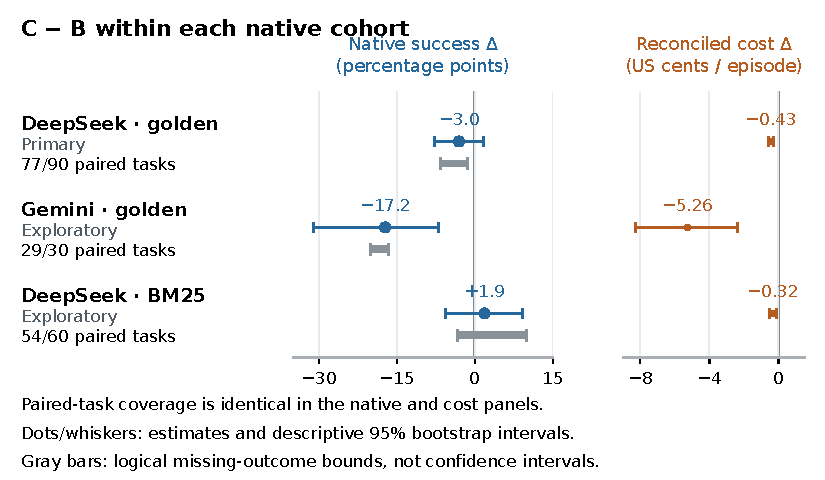
\includegraphics[width=\linewidth]{figures/native_c_minus_b_cost_success.pdf}
\caption{Within-cohort differences between typed-choice (C) and generative JSON (B)
gate-and-recovery bundles. Points and whiskers show equal-weight complete-task
means and descriptive 95\% task-bootstrap intervals; both panels use the same
task pairs. Gray bars bound native differences over the entire scheduled
cohort by assigning every unknown outcome both possible values. They measure
missing-outcome ambiguity, separately from bootstrap uncertainty. Primary
tasks retain three repeats per arm; exploratory tasks retain one. Costs
include all request roles on the qualified episode traces.}
\label{fig:v3-native-cost-effects}
\end{figure}

\paragraph{Reporting and admission amendments.}
The coordinator exposed interim descriptive comparisons and individual rewards
before final analysis, while confirmatory tests remained unexecuted. After
240 terminal primary slots and active-episode drain, a separately hashed and
tested reporting layer suppressed those outputs; earlier analyst access remains
unverified. After 647 terminal primary slots and coordinator drain, amendment
09 added transport diagnostics and an active-worker pause before new
reservations pending explicit accounting review. Activation recorded no pending
or unresolved attempts. Frozen core, original runner, plans and evidence were
preserved; samples, payloads, routes, scoring, error labels, alpha allocations
and caps remained fixed. Prior failures and unknown outcomes are retained.
Request timing starts after admission; pauses extend episode wall time.
Native-era ambiguous charges were subsequently reconciled; the affected native
outcomes remain unknown. Collection closed before the explicit guarded
analysis reported above.

\paragraph{Completed fixed-state probes.}
The synthetic bank covers identity evidence, verification time, a documented
bypass, exact email-change intent, referral expiry and referral terms. Six
scenarios per family yield 36 matched ternary triplets, or 108 states;
two judges and three repeats yielded 648 scheduled query attempts, all terminal. Closed-input predicates
and nested schema checks qualify this finite construction; unsupported shapes
are unscorable. Rule labels and provenance stay outside model input. The six
families are coverage units with dependent states and repeats; native
reachability is unestablished.

\autoref{tab:v3-rule-results} makes the tradeoff visible. C agreed more often
across repeated requests, yet matched fewer of the constructed policy labels.
Its complete three-repeat groups include 46 unanimous label errors, versus
nine for B. C allowed none of 106 qualified decisions on forbidden inputs, but
allowed 36/108 decisions on inputs missing required evidence and blocked
40/107 decisions on permitted inputs. B allowed all 106 qualified permitted-action
proposals, with two additional
unknowns. A low rate of approvals on explicitly forbidden states therefore
captures only one part of authorization performance.

\begin{table}[htbp]
\caption{Constructed policy-rule bank. Fractions use qualified decisions;
each gate has 324 scheduled requests. Agreement averages complete three-repeat
state groups, whose counts differ between gates. All results are descriptive.}
\label{tab:v3-rule-results}
\centering
\small
\begin{tabular}{@{}lrr@{}}
\toprule
Measure & B: LLM gate & C: typed-choice gate \\
\midrule
Qualified decisions / scheduled & 316/324 & 321/324 \\
Exact rule-label matches & 261/316 (82.6\%) & 175/321 (54.5\%) \\
Modal agreement; complete groups & 93.1\%; 101/108 & 98.7\%; 105/108 \\
Allow with missing evidence & 6/107 & 36/108 \\
Review with missing evidence & 56/107 & 2/108 \\
Allow when forbidden & 2/103 & 0/106 \\
Allow when permitted & 106/106 & 67/107 \\
Block when permitted & 0/106 & 40/107 \\
\bottomrule
\end{tabular}
\end{table}

Assigning every unknown either label-match outcome bounds B's scheduled
rule-label match at 80.6--83.0\% and C's at 54.0--54.9\%. These finite-bank bounds
retain all requests; neither the constructed labels nor repeated outputs
support population inference. Only 98 states have complete groups in both
gates, and cache freshness is unqualified.

Of 60 selected tasks in the natural-context study, nine supplied no audited
raw gate context and seven exceeded the frozen 90,000-byte common-admission
limit, leaving 44 contexts.
Four representations, three repeats and two gates yielded 1,056 terminal
query attempts: B returned 523/528
valid decisions and C 525/528. C-minus-B excess flips above each gate's
raw-repeat baseline were $+0.88$ pp for identifier renaming, $+8.33$ pp for
JSON syntax and $+10.00$ pp for both, on 38/44, 40/44 and 40/44 complete
paired tasks. Descriptive 95\% task-bootstrap intervals were
$[-7.02,+9.65]$, $[0.00,+17.50]$ and $[+0.83,+20.00]$ pp (2,000 draws).
Eight unavailable decisions leave the separate prespecified Holm(3) family at
$\alpha=0.025$ unavailable. These comparisons measure sensitivity to
representation, with no supplied policy-accuracy labels. Natural and synthetic
collection closed within their shared \$5 allocation.

\paragraph{A selected development case.}
In \texttt{task\_015}, B and C each
allowed a Business Gold referral-capability grant. The simulator used it and
ended satisfied, while native DB reward was zero. A obtained the date and
eventually supplied the reference program. Neither gate denied anything, and
generator behavior differed before intervention. Offline replay reproduced
captured DBs without a scoring discrepancy explaining the difference.
These unmatched pre-gate trajectories support an observational comparison;
causal gating effects require matched interventions.

Both gates saw the cutoff but no current time. The model-assisted interpretation
of native prose treats current program validity as a grant prerequisite,
mapping missing timing evidence to review. The observer's hidden clock is
separate from gate input; identity verification does not establish program
validity. Both raw inputs contain favorable generator
\texttt{reasoning\_details}. B's rationale discusses identity, provisioning
and terms but omits timing; C returns a choice and probabilities without an
explanation. This motivates shared-omission and self-justification hypotheses,
without identifying their causes: explanations can diverge from causal
computation, and distinct judges can share incomplete evidence. Confidence
thresholds cannot supply the missing fact.

The completed diagnostic crosses both original contexts, three timing states,
two rationale states, two judges and ten repeats: 12 visible states and
240 requests. Timing is missing, synthetically observed before the
unchanged cutoff, or observed after it. The dated pair differs only by date;
the missing comparison also adds a tool-call scaffold. Ablation removes only
the two generator \texttt{reasoning\_details} fields, preserving policy,
spoken content, intent and proposal. Changed information and length distinguish
this from nuisance invariance; persuasion is one possible explanation. Both
judges receive every variant. External labels assign review to missing timing
under the rubric and post-cutoff block under explicit policy; unclosed
prerequisites preclude unconditional pre-cutoff allow gold. A separate \$5
audit allocation bounds this diagnostic; cache freshness remains unqualified.

\autoref{fig:task015-evidence-boundary} shows all 24 cells. C allowed all
40 requests lacking a date. With a date after expiry, it allowed 18/20 requests
retaining the generator rationale, versus 1/20 after rationale removal.
B blocked all 40 after-expiry requests. Its missing-date cells contain
20 allows, three reviews and 17 unknown decisions. Another five unknowns
occur before expiry. All 22 unknowns are B output-limit failures: each used
4,096 completion tokens, with 21 responses allocating all of them to reasoning
and one returning an incomplete JSON prefix. Their concentration in missing-date
and pre-expiry cells makes qualified-only comparisons especially selective.

The completed expired-date cells show a concrete sensitivity to the retained
generator rationale. The ablation changes both information and input length,
so it leaves self-justification and other contextual explanations open.
The missing-date result separately shows that an available, repeatable choice
can still omit a prerequisite. These are observations on one selected task,
with no new native execution or population significance test.

\begin{figure}[t]
\centering
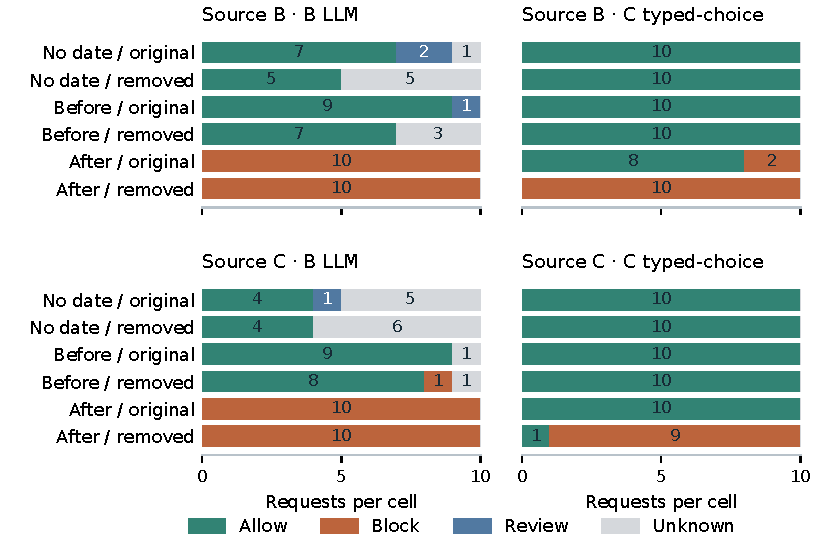
\includegraphics[width=\linewidth]{figures/task015-factorial-paper.pdf}
\caption{Selected referral diagnostic: 240 requests, 218 qualified decisions.
Rows vary the observed date and retain or remove generator rationale; columns
compare both judges on the same visible states from two related source
contexts. Before/after refer to the unchanged program-expiry cutoff.
Missing-date review follows the stated rubric; after-expiry block follows the
temporal rule. Unknowns retain unavailable decisions in each ten-request cell.
The two source contexts belong to one development task.}
\label{fig:task015-evidence-boundary}
\end{figure}

\paragraph{Architecture, economics and selective calibration.}
Models propose and assess, code enforces constraints, and traces connect evidence,
permission and effect. Execution-monitoring limits and three-valued semantics
provide prior foundations~\citep{schneider2000enforceable,bauer2011runtime}.
TypeSafe documents date-ordering, distracting-context and adversarial-content
weaknesses, recommending code for date comparisons~\citep{typesafe2026jevdocs};
such a date check would be a separately specified intervention retaining unknown
inputs. Harness search and runtime-governance studies remain related work,
not evaluated interventions here~\citep{liu2026solpi,shlomov2026governance}.

LangChain describes Jev routing and tool-risk middleware; its evaluator study
uses five fixed weather-agent outputs judged 100 times each, so those five
outputs are the units~\citep{runkle2026harness,shea2026jevjudge}. Its archived
analysis reports lower Jev repeated-score variance, while other judges have
lower continuous-quality mean absolute error against additional oracle scores
(\hyperref[app:artifact]{Appendix~\ref*{app:artifact}}). Different score
constructions limit mechanistic interpretation: consistency may repeat a bias.
Authorization evaluation must identify stable errors and their permitted or
prevented actions.

Calibration requires target-workload validation; distribution shift can
undermine uncertainty estimates~\citep{guo2017calibration,ovadia2019uncertainty}.
TypeSafe recommends domain-specific threshold validation for its
class-probability confidence~\citep{typesafe2026jevdocs}; policy-compliance and absence-of-harm
probabilities require separate validation. Frozen C uses categorical choice.
Natural per-action calibration needs independent policy labels; rule-bank
diagnostics retain constructed-label scope.

Cost per native success is undefined at zero successes, and safety-qualified completion has
a separate denominator. Unsupported permissions, false blocks, review,
recovery and native completion carry distinct consequences. Request, wrapper
and workflow timing retain separate boundaries; campaign wall time accounts
for concurrency.

\autoref{fig:development-request-cost} describes six rules-only development
cohorts' generator/simulator latency and API cost, without gate or grader
calls and with differing task/configuration mixes.
\hyperref[app:deployment]{Appendix~\ref*{app:deployment}} retains the separate
Ollama technical qualification, local memory and ownership-cost scenarios.
Cost is assessed alongside evidence, permitted-action coverage and outcomes.
